% -----------------------------------------------
% Template for ISMIR Papers
% 2016 version, based on previous ISMIR templates

% Requirements :
% * 6+1 page length maximum
% * 2MB maximum file size
% * Copyright note must appear in the bottom left corner of first page
% (see conference website for additional details)
% -----------------------------------------------

\documentclass{article}
\usepackage{ismir,amsmath,cite}
\usepackage{graphicx}
\usepackage{color}

% Title.
% ------
\title{Beat Phase Modeling with Laplacian Circular Coordinates}

% Note: Please do NOT use \thanks or a \footnote in any of the author markup

% Single address
% To use with only one author or several with the same address
% ---------------
%\oneauthor
% {Names should be omitted for double-blind reviewing}
% {Affiliations should be omitted for double-blind reviewing}

% Two addresses
% --------------
%\twoauthors
%  {First author} {School \\ Department}
%  {Second author} {Company \\ Address}

%% To make customize author list in Creative Common license, uncomment and customize the next line
%  \def\authorname{First Author, Second Author} 


% Three addresses
% --------------
\oneauthor
  {Christopher J. Tralie} {Duke University Department of Electrical And Computer Engineering \\ {\tt chris.tralie@gmail.com}}

%% To make customize author list in Creative Common license, uncomment and customize the next line
%  \def\authorname{First Author, Second Author, Third Author} 

% Four or more addresses
% OR alternative format for large number of co-authors
% ------------
%\multauthor
%{First author$^1$ \hspace{1cm} Second author$^1$ \hspace{1cm} Third author$^2$} { \bfseries{Fourth author$^3$ \hspace{1cm} Fifth author$^2$ \hspace{1cm} Sixth author$^1$}\\
%  $^1$ Department of Computer Science, University , Country\\
%$^2$ International Laboratories, City, Country\\
%$^3$  Company, Address\\
%{\tt\small CorrespondenceAuthor@ismir.edu, PossibleOtherAuthor@ismir.edu}
%}
%\def\authorname{First author, Second author, Third author, Fourth author, Fifth author, Sixth author}


\sloppy % please retain sloppy command for improved formatting

\begin{document}

%
\maketitle
%
\begin{abstract}
In this work, we introduce a geometric technique for automatically modeling musical audio {\em beat phase}, which is the distance of each audio sample to the next occurring beat onset.  We show that sliding window embeddings of typical audio novelty functions form topological loops in the sliding window embedding space, and we use the principal components of these embeddings to visualize and animate beats as they evolve.  For more precise estimates of beat phase, we build a nearest neighbor graph in the sliding window embedding space, and we use the eigenvectors corresponding to the two smallest nonzero eigenvalues of the graph Laplacian to put circular coordinates on each window, which can be post-processed into a continuous estimate of beat phase.  A dynamic programming algorithm can then be used to extract beat onsets by trading off audio novelty and closeness of inter-onset-intervals to one full revolution of the circle.  At this stage, it is also possible to model multiscale tempo hierarchies, and we provide a double pendulum GUI to visualize this.  %We report state of the art results both in beat onset detection and tempo estimation using this technique.
\end{abstract}
%
\section{Introduction}\label{sec:introduction}

Automatic beat tracking in musical audio is a surprisingly difficult problem due to the highly dynamic nature of music.  Many transient events occur in a short amount of time which can distract from the main beat onsets, so naive techniques that do peak picking in an energy differential function are doomed to fail.  A litany of sophisticated work has addressed this

In this work, we provide a different perspective on this problem.  We use tools from nonlinear time series analysis to cast the problem of beat modeling as tracing curves around loops in high dimensions.   

\section{Background}

Talk about novelty functions, beat tracking techniques

Define map from audio to the circle

\section{Sliding Windows on Novelty Functions}

\subsection{Geometry of Sliding Windows of Periodic Functions}

Show SSM and PCA on audio novelty functions

\subsection{Face Jam GUI}

\subsection{Sliding window denoising}


\section{Laplacian Circular Coordinates}

\subsection{Graph Laplacians}

\subsection{Merging Sliding Window Blocks}

\subsection{Metrical Hierarchies / Pendulum GUI}


\section{Dynamic Programming Onset Extraction}


\section{Beat Tracking Evaluation}

%\begin{table}
% \begin{center}
% \begin{tabular}{|l|l|}
%  \hline
%  String value & Numeric value \\
%  \hline
%  Hello ISMIR  & \conferenceyear \\
%  \hline
% \end{tabular}
%\end{center}
% \caption{Table captions should be placed below the table.}
% \label{tab:example}
%\end{table}

%\begin{figure}
% \centerline{\framebox{
% 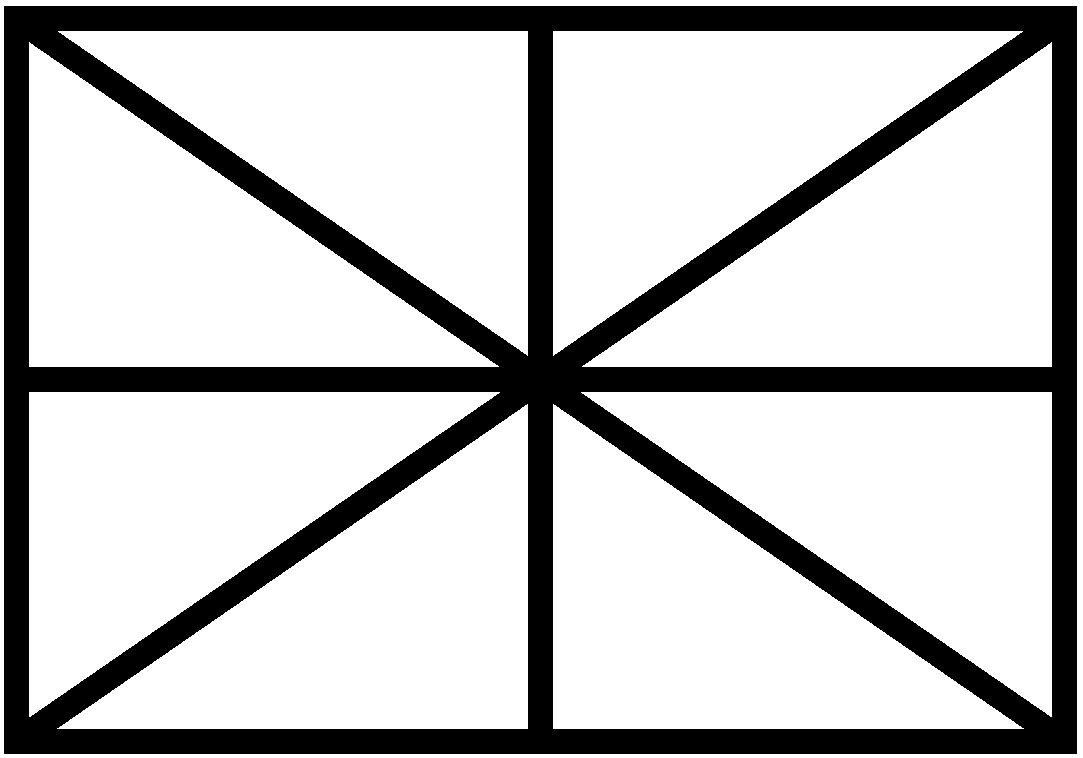
\includegraphics[width=\columnwidth]{figure.png}}}
% \caption{Figure captions should be placed below the figure.}
% \label{fig:example}
%\end{figure}



% For bibtex users:
\bibliography{LaplacianBeatTracking}


\end{document}
